Figure~\ref{fig:metamodel} summarizes all presented approaches with design patterns and the relations between them.

\begin{figure}[!htb]
    \centering
    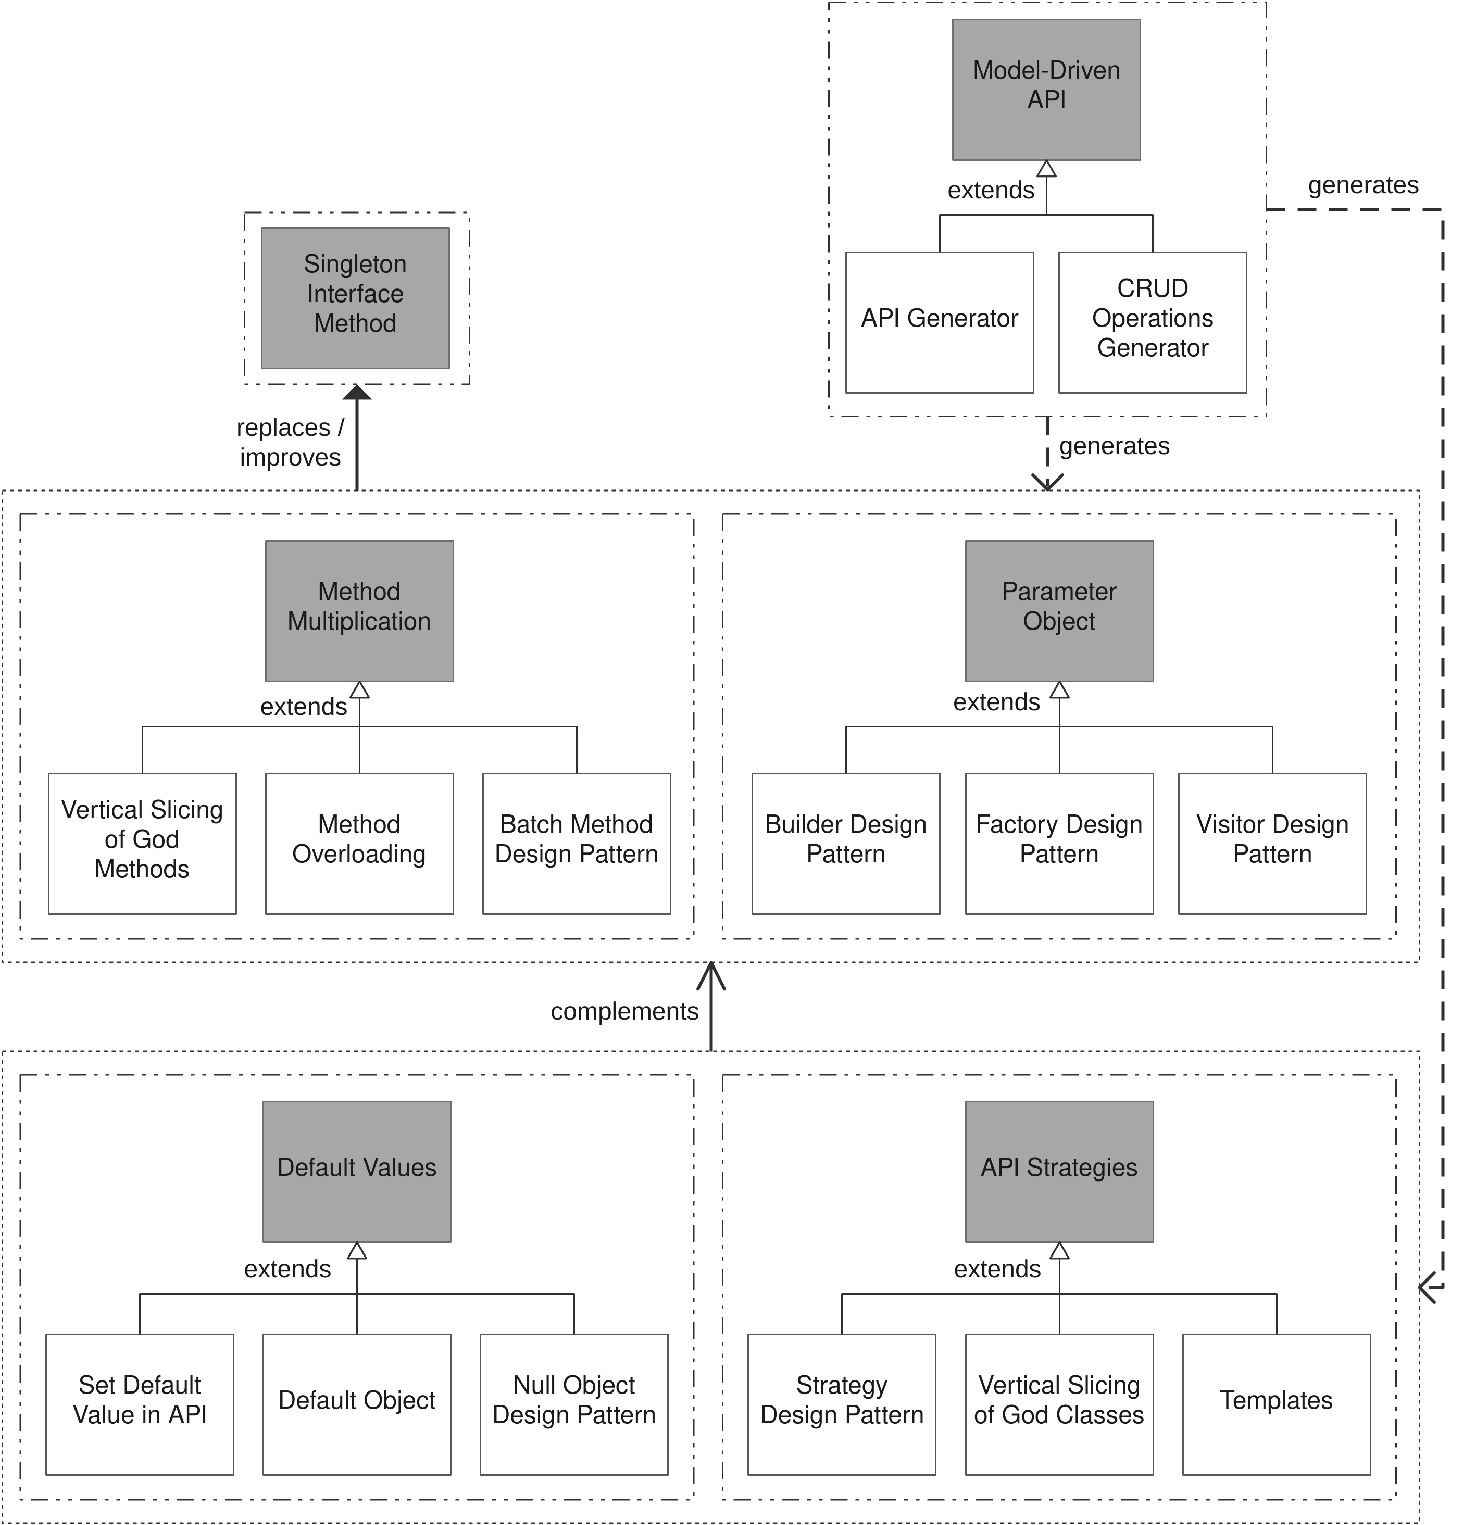
\includegraphics[width=1.0
    \textwidth]{metamodel}
    \caption{Summary: Metamodel containing overview of presented approaches and patterns}
    \label{fig:metamodel}
\end{figure}

The guide starts with the Singleton Interface Method, which is the most basic approach for modeling internal
synchronous APIs.
This modeling approach is suitable for simple methods without the need for flexibility and extensibility.
However, there are many cases when this approach is not suitable, and more advanced design patterns are required
to preserve code quality.

The Method Multiplication focuses on the vertical slicing of interface methods into more granular interface methods,
thus breaking God Methods that usually occur in Singleton Interface Methods.
On the other side, the Default Values approach does not try to break methods into smaller pieces but rather aims
to reduce the number of methods by providing default values for optional parameters.
From the view of the metamodel, both Method Multiplication and Default Values are successors
of the Singleton Interface Method when dealing with a more complex API with more responsibilities
or expectations for API evolution.

The Parameter Object represents the next design pattern that can be used for the simplification of method signatures
and reusability of a group of parameters.
There are multiple ways to construct a Parameter Object, for example, using Builder or Factory design patterns.
It is also possible to construct more complex Parameter Objects by aggregating other objects
or introducing inheritance between different types of Parameter Objects.

The API Strategies approach goes beyond Method Multiplication and extends the vertical slicing of interface methods
by introducing different API subtypes.
This is handy if there is a need to provide a similar API for different data types or in different contexts.
Parameter Object and API Strategies are most often used as the next step in the design or refactoring process
after Method Multiplication or Default Values are applied but still not enough to achieve
the desired decomposition level.
All of these approaches and design patterns are not mutually exclusive and can be used together.

The final section presents the concept of Model-Driven API, which is based on the idea of defining the model
and generating API interfaces and entities from the model.
The generation of API ensures consistency and reduces the amount of boilerplate code.
However, it also introduces additional complexity and dependency on the model and tools.
Because of this, it is usually used for external APIs connecting different services and clients.
